In this Chapter we compare performances of our method against a number of different baselines on
a series of different problems. The algorithms we compare against are POMCP, RTBSS and a belief
based RTBSS (which we refer to as RTBSSb).

RTBSS is an online branch-and-bound solver for POMDPs, which enumerates every possible outcome from
a given state for a given horizon, and thus computes the true value function for that state and
the best action that can be performed. RTBSSb works in the same way, but it computes rewards using a
given belief-based reward function. RTBSS trades its precision and accuracy with speed: since it has
to explore most of the possible outcomes, the size of problems it can handle is limited.

Even though POMCP and RTBSS are algorithms which require a state-based reward function, we can
compare them against the performance of max-of-belief rPOMCP. This is possible since a max-of-belief
reward function can be converted into a state-based reward function by modifying the action space of
the problem. In the new action space, each action represents at the same time one of the old
actions, plus an addictional \textit{prediction action}, which is used by the agent in order to
predict the state the environment is in at any given time. The new action space is thus the result
of a cross-product between the set of old actions and the new prediction actions, which are $|S|$.

\ys{be consistent with the framework you are using. Stick to rho POMDP, no need for prediction actions}

The reward function is then defined in terms of the prediction actions: if the agent predicts the
state of the environment correctly, it receives a reward of 1. Otherwise, it receives no reward. It
follows that the expected returns with the new reward function are the same than that of a
max-of-belief reward function, as the agent will guess the state of the environment correctly with a
rate equal to the maximum of its belief.

The disadvantage of this transformation is that the action space becomes exponentially bigger the
more states are available, which significantly impairs both POMCP and RTBSS.

RTBSSb can instead be applied directly on both max-of-belief and entropy based rewards.

\section{First Model - Simple Environment}

In this section we apply the proposed algorithms to the following model: a single target walking
between six rooms. The target can be at any time in a single room, and can transition between them
as showed in \ref{ref:nonmyo1}. The agent can observe, at each timestep, whether the target is in a
given room. The information gathered by the agent will be correct with probability $p=0.8$. In each
episode the target starts in a random room, and the agent goal is to track it for 10 timesteps. The
agent receives a reward of 1 if it can correctly guess the position of the target, and 0 otherwise.
This problem is also discussed in Appendix \ref{ref:appendix_proof} to show how a non-myopic
approach can be preferred over a myopic one.

\begin{figure}[ht]
\centering
\begin{tikzpicture}[->,>=stealth',shorten >=1pt,auto,node distance=4cm,thick,main node/.style={circle,draw,font=\Large\bfseries}]
\tikzstyle{state} = [circle, draw=black, fill=green!30]
\tikzstyle{arrow} = [thick,->,>=stealth]

\node (s1) at (0,0) [state] {S1};
\node (s2) at (2,3) [state] {S2};
\node (s3) at (4,0) [state] {S3};
\node (s4) at (6,0) [state] {S4};
\node (s5) at (8,3) [state] {S5};
\node (s6) at (10,0) [state] {S6};

\path
    (s1) edge [loop below] node {0.333} (s1)
         edge [bend left] node {0.333} (s2)
         edge [bend left=10] node[below] {0.333} (s3)
    (s2) edge [loop above] node {0.333} (s2)
         edge [bend left=10] node[above,rotate=60] {0.333} (s1)
         edge [bend left] node {0.333} (s3)
    (s3) edge [loop below] node {0.333} (s3)
         edge [bend left=10] node[above,rotate=-60] {0.333} (s2)
         edge [bend left] node {0.333} (s1)
    (s4) edge [bend left] node {1.0} (s5)
    (s5) edge [bend left] node {1.0} (s6)
    (s6) edge [bend left] node {1.0} (s4);

\end{tikzpicture}
\caption{The graphical representation of our first model.}
\label{ref:nonmyo1}
\end{figure}

Figure \ref{ref:myoentropyfig} and Figure \ref{ref:myombfig} show performance in terms of cumulative
obtained reward for the different methods proposed. We also compare performances of POMCP/rPOMCP
using different number of samples. In addition, we test rPOMCP with different $k$ parameters, tuning
the mean-max backup operation towards one or the other. $k = 1$ results in a max backup
operation, while $k = 10000$ results in an essentially mean backup operation of values.

The $h$ parameter determines the horizon of the particular solver. $h = 1$ results in a greedy
solver. It is important to note that for POMCP and rPOMCP $h$ is merely an upper bound on the depth
of the decision tree they are allowed to explore. This is because they build their decision tree
incrementally, so that they may not reach its true bottom of their decision tree if the number of
samples is not sufficient.

\begin{figure}[ht]
        \centering
        \begin{subfigure}[t]{0.3\textwidth}
                \includegraphics[width=\textwidth]{Images/MyoResults/1e4/E/output}
                \caption{Results using 1e4 samples.}
                \label{fig:m4e}
        \end{subfigure}%
        ~ %add desired spacing between images, e. g. ~, \quad, \qquad, \hfill etc.
          %(or a blank line to force the subfigure onto a new line)
        \begin{subfigure}[t]{0.3\textwidth}
                \includegraphics[width=\textwidth]{Images/MyoResults/1e5/E/output}
                \caption{Results using 1e5 samples.}
                \label{fig:m5e}
        \end{subfigure}
        ~ %add desired spacing between images, e. g. ~, \quad, \qquad, \hfill etc.
          %(or a blank line to force the subfigure onto a new line)
        \begin{subfigure}[t]{0.3\textwidth}
                \includegraphics[width=\textwidth]{Images/MyoResults/1e6/E/output}
                \caption{Results using 1e6 samples.}
                \label{fig:m6e}
        \end{subfigure}
        \caption{Results in our first model using entropy, averaged over 3000 episodes.}
        \label{ref:myoentropyfig}
\end{figure}

\ys{I think there are too many lines in this figures. For showing the performance with increasing number of samples, you can fix k = 1 or 1000, fix a horizon to 5 or 2 and then you can increase number of samples to show variations.}


\begin{figure}[ht!]
        \centering
        \begin{subfigure}[t]{0.3\textwidth}
                \includegraphics[width=\textwidth]{Images/MyoResults/1e4/MB/output}
                \caption{Results using 1e4 samples.}
                \label{fig:m4m}
        \end{subfigure}%
        ~ %add desired spacing between images, e. g. ~, \quad, \qquad, \hfill etc.
          %(or a blank line to force the subfigure onto a new line)
        \begin{subfigure}[t]{0.3\textwidth}
                \includegraphics[width=\textwidth]{Images/MyoResults/1e5/MB/output}
                \caption{Results using 1e5 samples.}
                \label{fig:m5m}
        \end{subfigure}
        ~ %add desired spacing between images, e. g. ~, \quad, \qquad, \hfill etc.
          %(or a blank line to force the subfigure onto a new line)
        \begin{subfigure}[t]{0.3\textwidth}
                \includegraphics[width=\textwidth]{Images/MyoResults/1e6/MB/output}
                \caption{Results using 1e6 samples.}
                \label{fig:m6m}
        \end{subfigure}
        \caption{Results in our first model using max-of-belief, averaged over 3000 episodes.}
        \label{ref:myombfig}
\end{figure}

\ys{there is no need probably to show how max of belief/entropy differs with number of sample, unless the behaviour is extremely different. Instead you can compare the performance between max of belief and entropy by fixing number of sample, k and h and then show how max of belief/entropy matters}.

We can see how a small horizon always results in a lower return over the 10 timesteps. This is
because with a greedy approach the agent cannot leverage the fact that half of the environment is
deterministic, and thus more useful to explore beforehand. This is most visible in the max-of-belief
setting, while the entropy reward function does not suffer from a significant loss of performance.

\clearpage
\section{Second Model - Finite Budget}

In this Section we apply the proposed algorithms to the following model: a 4-room world where a
target can transition, at each timestep, from a room to any of the two rooms adjacent. The
observation and reward function follow the logic of our first model: the agent can observe a single
room at a time, and needs to keep track of the target for 15 timesteps. The target here always
starts from a given room, known to the agent.

In this model there is an additional rule: the agent is only allowed to look at the world 4 times;
after that each action will yield no additional information. The agent can, at each timestep, decide
whether to use one of its observations, or save them for a future timestep. This last constraint is
used to simulate real-life resource constraints; for example when energy and/or processing
constraints limit the number of times a multi-camera system is allowed to observe the environment.

The idea is that the agent should use up an observation only if has low knowledge about the world;
otherwise it should keep its observation actions for later.

\begin{figure}[ht]
\centering
\begin{tikzpicture}[->,>=stealth',shorten >=1pt,auto,node distance=4cm,thick,main node/.style={circle,draw,font=\Large\bfseries}]
\tikzstyle{state} = [circle, draw=black, fill=green!30]
\tikzstyle{arrow} = [thick,<->,>=stealth]

\node (s1) at (0,3) [state] {S1};
\node (s2) at (3,3) [state] {S2};
\node (s3) at (0,0) [state] {S3};
\node (s4) at (3,0) [state] {S4};

\path
    (s1) edge [arrow] node {0.5} (s2)
    (s2) edge [arrow] node {0.5} (s4)
    (s3) edge [arrow] node {0.5} (s1)
    (s4) edge [arrow] node {0.5} (s3);

\end{tikzpicture}
\caption{The graphical representation of our second model.}
\label{ref:finbudget1}
\end{figure}

We tested this model in two configurations: one where the target transitions randomly between the
two rooms available, increasing maximally the entropy at each timestep, and one where the target
transitions to its left with a probability of $0.75$. This was done in order to see how the agent behavior
changed with respect to a differently predictable target.

\begin{figure}[ht]
        \centering
        \begin{subfigure}[t]{0.3\textwidth}
                \includegraphics[width=\textwidth]{Images/FiniteBudgetResults/0.5/1e4/E/output}
                \caption{Results using 1e4 samples.}
                \label{fig:fb4e5}
        \end{subfigure}%
        ~ %add desired spacing between images, e. g. ~, \quad, \qquad, \hfill etc.
          %(or a blank line to force the subfigure onto a new line)
        \begin{subfigure}[t]{0.3\textwidth}
                \includegraphics[width=\textwidth]{Images/FiniteBudgetResults/0.5/1e5/E/output}
                \caption{Results using 1e5 samples.}
                \label{fig:fb5e5}
        \end{subfigure}
        ~ %add desired spacing between images, e. g. ~, \quad, \qquad, \hfill etc.
          %(or a blank line to force the subfigure onto a new line)
        \begin{subfigure}[t]{0.3\textwidth}
                \includegraphics[width=\textwidth]{Images/FiniteBudgetResults/0.5/1e6/E/output}
                \caption{Results using 1e6 samples.}
                \label{fig:fb6e5}
        \end{subfigure}
        \caption{Results in the Finite Budget model with a transition factor of 0.5, using entropy, averaged over 3000 episodes.}
        \label{ref:fbentropyfig5}
\end{figure}

\begin{figure}[ht]
        \centering
        \begin{subfigure}[t]{0.3\textwidth}
                \includegraphics[width=\textwidth]{Images/FiniteBudgetResults/0.5/1e4/MB/output}
                \caption{Results using 1e4 samples.}
                \label{fig:fb4m5}
        \end{subfigure}%
        ~ %add desired spacing between images, e. g. ~, \quad, \qquad, \hfill etc.
          %(or a blank line to force the subfigure onto a new line)
        \begin{subfigure}[t]{0.3\textwidth}
                \includegraphics[width=\textwidth]{Images/FiniteBudgetResults/0.5/1e5/MB/output}
                \caption{Results using 1e5 samples.}
                \label{fig:fb5m5}
        \end{subfigure}
        ~ %add desired spacing between images, e. g. ~, \quad, \qquad, \hfill etc.
          %(or a blank line to force the subfigure onto a new line)
        \begin{subfigure}[t]{0.3\textwidth}
                \includegraphics[width=\textwidth]{Images/FiniteBudgetResults/0.5/1e6/MB/output}
                \caption{Results using 1e6 samples.}
                \label{fig:fb6m5}
        \end{subfigure}
        \caption{Results in the Finite Budget model with a transition factor of 0.5, using max-of-belief, averaged over 3000 episodes.}
        \label{ref:fbmbfig5}
\end{figure}

\begin{figure}[ht]
        \centering
        \begin{subfigure}[t]{0.3\textwidth}
                \includegraphics[width=\textwidth]{Images/FiniteBudgetResults/0.75/1e4/E/output}
                \caption{Results using 1e4 samples.}
                \label{fig:fb4e75}
        \end{subfigure}%
        ~ %add desired spacing between images, e. g. ~, \quad, \qquad, \hfill etc.
          %(or a blank line to force the subfigure onto a new line)
        \begin{subfigure}[t]{0.3\textwidth}
                \includegraphics[width=\textwidth]{Images/FiniteBudgetResults/0.75/1e5/E/output}
                \caption{Results using 1e5 samples.}
                \label{fig:fb5e75}
        \end{subfigure}
        ~ %add desired spacing between images, e. g. ~, \quad, \qquad, \hfill etc.
          %(or a blank line to force the subfigure onto a new line)
        \begin{subfigure}[t]{0.3\textwidth}
                \includegraphics[width=\textwidth]{Images/FiniteBudgetResults/0.75/1e6/E/output}
                \caption{Results using 1e6 samples.}
                \label{fig:fb6e75}
        \end{subfigure}
        \caption{Results in the Finite Budget model with a transition factor of 0.75, using entropy, averaged over 3000 episodes.}
        \label{ref:fbentropyfig75}
\end{figure}

\begin{figure}[ht]
        \centering
        \begin{subfigure}[t]{0.3\textwidth}
                \includegraphics[width=\textwidth]{Images/FiniteBudgetResults/0.75/1e4/MB/output}
                \caption{Results using 1e4 samples.}
                \label{fig:fb4m75}
        \end{subfigure}%
        ~ %add desired spacing between images, e. g. ~, \quad, \qquad, \hfill etc.
          %(or a blank line to force the subfigure onto a new line)
        \begin{subfigure}[t]{0.3\textwidth}
                \includegraphics[width=\textwidth]{Images/FiniteBudgetResults/0.75/1e5/MB/output}
                \caption{Results using 1e4 samples.}
                \label{fig:fb5m75}
        \end{subfigure}
        ~ %add desired spacing between images, e. g. ~, \quad, \qquad, \hfill etc.
          %(or a blank line to force the subfigure onto a new line)
        \begin{subfigure}[t]{0.3\textwidth}
                \includegraphics[width=\textwidth]{Images/FiniteBudgetResults/0.75/1e6/MB/output}
                \caption{Results using 1e4 samples.}
                \label{fig:fb6m75}
        \end{subfigure}
        \caption{Results in the Finite Budget model with a transition factor of 0.75, using max-of-belief, averaged over 3000 episodes.}
        \label{ref:fbmbfig75}
\end{figure}

\ys{I think it applied for most of the figures here, there is no need to have so many parameters change in each graph. Fix everything else and just change one parameter and tell what is the take away message from changing that parameter}.


\clearpage
\section{Third Model - Realistic Scenario}

In this Section we test rPOMCP on yet another model. Here the target can walk in a grid world, in a
north-south-east-west fashion. To produce a somewhat realistic environment, the target selects a
random cell at any time, and then moves towards it. Once it reaches it, it selects another goal
cell, and continues. However, the agent's model of the environment does not include this: the agent
only knows that the target can move randomly towards an adjacent cell. The target always starts from
the center of the grid, with the agent knowing it.

The world is observed by cameras, where each camera can observe a 5x5 patch of the overall world.
Each camera can observe imperfectly: the closer the target is towards the center of the patch, the
more accurate the observations will be. Otherwise the camera will report the target on any cell
adjacent to the true target. If the reported cell is outside the camera range, the camera will not
report observing the target.

The agent is allowed to use a single camera at the time, and again needs to keep track of the target
over 75 timesteps.

We show results with two different versions of the world: a small 20x20 environment, and a bigger
50x50 one. Due to the big number of states, POMCP and RTBSS cannot be used here; RTBSSb can be
barely used with a greedy horizon for the small environment.

\begin{figure}[ht]
        \centering
        \begin{subfigure}[t]{0.3\textwidth}
                \includegraphics[width=\textwidth]{Images/CameraBasicResults/Small_20x20/1e4/E/output}
                \caption{Results using 1e4 samples.}
                \label{fig:cws4e}
        \end{subfigure}%
        ~ %add desired spacing between images, e. g. ~, \quad, \qquad, \hfill etc.
          %(or a blank line to force the subfigure onto a new line)
        \begin{subfigure}[t]{0.3\textwidth}
                \includegraphics[width=\textwidth]{Images/CameraBasicResults/Small_20x20/1e6/E/output}
                \caption{Results using 1e5 samples.}
                \label{fig:cws5e}
        \end{subfigure}
        ~ %add desired spacing between images, e. g. ~, \quad, \qquad, \hfill etc.
          %(or a blank line to force the subfigure onto a new line)
        \begin{subfigure}[t]{0.3\textwidth}
                \includegraphics[width=\textwidth]{Images/CameraBasicResults/Small_20x20/1e6/E/output}
                \caption{Results using 1e6 samples.}
                \label{fig:cws6e}
        \end{subfigure}
        \caption{Results in our realistic model using a 20x20 grid, using entropy, averaged over 3000 episodes.}\label{fig:cwse}
\end{figure}

\begin{figure}[ht]
        \centering
        \begin{subfigure}[t]{0.3\textwidth}
                \includegraphics[width=\textwidth]{Images/CameraBasicResults/Small_20x20/1e4/MB/output}
                \caption{Results using 1e4 samples.}
                \label{fig:cws4mb}
        \end{subfigure}%
        ~ %add desired spacing between images, e. g. ~, \quad, \qquad, \hfill etc.
          %(or a blank line to force the subfigure onto a new line)
        \begin{subfigure}[t]{0.3\textwidth}
                \includegraphics[width=\textwidth]{Images/CameraBasicResults/Small_20x20/1e6/MB/output}
                \caption{Results using 1e5 samples.}
                \label{fig:cws5mb}
        \end{subfigure}
        ~ %add desired spacing between images, e. g. ~, \quad, \qquad, \hfill etc.
          %(or a blank line to force the subfigure onto a new line)
        \begin{subfigure}[t]{0.3\textwidth}
                \includegraphics[width=\textwidth]{Images/CameraBasicResults/Small_20x20/1e6/MB/output}
                \caption{Results using 1e6 samples.}
                \label{fig:cws6mb}
        \end{subfigure}
        \caption{Results in our realistic model using a 20x20 grid, using max-of-belief, averaged over 3000 episodes.}\label{fig:cwsmb}
\end{figure}

\begin{figure}[ht]
        \centering
        \begin{subfigure}[t]{0.3\textwidth}
                \includegraphics[width=\textwidth]{Images/CameraBasicResults/Big_50x50/1e4/E/output}
                \caption{Results using 1e4 samples.}
                \label{fig:cwb4e}
        \end{subfigure}%
        ~ %add desired spacing between images, e. g. ~, \quad, \qquad, \hfill etc.
          %(or a blank line to force the subfigure onto a new line)
        \begin{subfigure}[t]{0.3\textwidth}
                \includegraphics[width=\textwidth]{Images/CameraBasicResults/Big_50x50/1e6/E/output}
                \caption{Results using 1e5 samples.}
                \label{fig:cwb5e}
        \end{subfigure}
        ~ %add desired spacing between images, e. g. ~, \quad, \qquad, \hfill etc.
          %(or a blank line to force the subfigure onto a new line)
        \begin{subfigure}[t]{0.3\textwidth}
                \includegraphics[width=\textwidth]{Images/CameraBasicResults/Big_50x50/1e6/E/output}
                \caption{Results using 1e6 samples.}
                \label{fig:cwb6e}
        \end{subfigure}
        \caption{Results in our realistic model using a 50x50 grid, using entropy, averaged over 3000 episodes.}\label{fig:cwbe}
\end{figure}

\begin{figure}[ht]
        \centering
        \begin{subfigure}[t]{0.3\textwidth}
                \includegraphics[width=\textwidth]{Images/CameraBasicResults/Big_50x50/1e4/MB/output}
                \caption{Results using 1e4 samples.}
                \label{fig:cwb4mb}
        \end{subfigure}%
        ~ %add desired spacing between images, e. g. ~, \quad, \qquad, \hfill etc.
          %(or a blank line to force the subfigure onto a new line)
        \begin{subfigure}[t]{0.3\textwidth}
                \includegraphics[width=\textwidth]{Images/CameraBasicResults/Big_50x50/1e6/MB/output}
                \caption{Results using 1e5 samples.}
                \label{fig:cwb5mb}
        \end{subfigure}
        ~ %add desired spacing between images, e. g. ~, \quad, \qquad, \hfill etc.
          %(or a blank line to force the subfigure onto a new line)
        \begin{subfigure}[t]{0.3\textwidth}
                \includegraphics[width=\textwidth]{Images/CameraBasicResults/Big_50x50/1e6/MB/output}
                \caption{Results using 1e6 samples.}
                \label{fig:cwb6mb}
        \end{subfigure}
        \caption{Results in our realistic model using a 50x50 grid, using max-of-belief, averaged over 3000 episodes.}\label{fig:cwbmb}
\end{figure}

In Figure \ref{fig:cwb10} we show the results of applying rPOMCP to a multi-tracking scenario, where
10 targets are allowed to roam the grid world concurrently. In this experiment, we run 10 instances
of rPOMCP in a parallel fashion, one for each target. These 10 instances approximate values for
every possible action, given their belief on their respective target. At every timestep, the action that
maximizes overall value over all rPOMCP instances is chosen.

\begin{figure}[ht!]
        \centering
        \begin{subfigure}[t]{0.5\textwidth}
                \includegraphics[width=\textwidth]{Images/CameraBasicResults/Big_50x50/Multi/E/output}
                \caption{Results using 1e4 samples and entropy.}
                \label{fig:cwb4e10}
        \end{subfigure}%
        ~ %add desired spacing between images, e. g. ~, \quad, \qquad, \hfill etc.
          %(or a blank line to force the subfigure onto a new line)
        \begin{subfigure}[t]{0.5\textwidth}
                \includegraphics[width=\textwidth]{Images/CameraBasicResults/Big_50x50/Multi/MB/output}
                \caption{Results using 1e4 samples and max-of-belief.}
                \label{fig:cwb5mb10}
        \end{subfigure}
        \caption{Results in our realistic model 50x50 tracking 10 unique targets, averaged over 3000 episodes.}\label{fig:cwb10}
\end{figure}

In addition to the previous experiments, we also created a separate model where the agent's model of
the target movements is improved. In this second version of Camera World, the model keeps track of
the previous direction that the target moved, and predicts a $0.7$ probability that the target will
continue to move in the same direction, or randomly otherwise. This is done by increasing the state
space by four times, where each state now encodes a previous target direction and the target current
position.

In this new model unfortunately RTBSSb cannot be used, as the state space is too big and RTBSSb
takes too much time to complete.

\begin{figure}[ht!]
        \centering
        \begin{subfigure}[t]{0.3\textwidth}
                \includegraphics[width=\textwidth]{Images/CameraPathResults/Small_20x20/1e4/E/output}
                \caption{Results using 1e4 samples.}
                \label{fig:cps4e}
        \end{subfigure}%
        ~ %add desired spacing between images, e. g. ~, \quad, \qquad, \hfill etc.
          %(or a blank line to force the subfigure onto a new line)
        \begin{subfigure}[t]{0.3\textwidth}
                \includegraphics[width=\textwidth]{Images/CameraPathResults/Small_20x20/1e6/E/output}
                \caption{Results using 1e5 samples.}
                \label{fig:cps5e}
        \end{subfigure}
        ~ %add desired spacing between images, e. g. ~, \quad, \qquad, \hfill etc.
          %(or a blank line to force the subfigure onto a new line)
        \begin{subfigure}[t]{0.3\textwidth}
                \includegraphics[width=\textwidth]{Images/CameraPathResults/Small_20x20/1e6/E/output}
                \caption{Results using 1e6 samples.}
                \label{fig:cps6e}
        \end{subfigure}
        \caption{Results in the Camera World 2 20x20, using entropy, averaged over 3000 episodes.}\label{fig:cpse}
\end{figure}

\begin{figure}[ht]
        \centering
        \begin{subfigure}[t]{0.3\textwidth}
                \includegraphics[width=\textwidth]{Images/CameraPathResults/Small_20x20/1e4/MB/output}
                \caption{Results using 1e4 samples.}
                \label{fig:cps4mb}
        \end{subfigure}%
        ~ %add desired spacing between images, e. g. ~, \quad, \qquad, \hfill etc.
          %(or a blank line to force the subfigure onto a new line)
        \begin{subfigure}[t]{0.3\textwidth}
                \includegraphics[width=\textwidth]{Images/CameraPathResults/Small_20x20/1e6/MB/output}
                \caption{Results using 1e5 samples.}
                \label{fig:cps5mb}
        \end{subfigure}
        ~ %add desired spacing between images, e. g. ~, \quad, \qquad, \hfill etc.
          %(or a blank line to force the subfigure onto a new line)
        \begin{subfigure}[t]{0.3\textwidth}
                \includegraphics[width=\textwidth]{Images/CameraPathResults/Small_20x20/1e6/MB/output}
                \caption{Results using 1e6 samples.}
                \label{fig:cps6mb}
        \end{subfigure}
        \caption{Results in the Camera World 2 20x20, using entropy, averaged over 3000 episodes.}\label{fig:cpsmb}
\end{figure}

\begin{figure}[ht]
        \centering
        \begin{subfigure}[t]{0.3\textwidth}
                \includegraphics[width=\textwidth]{Images/CameraPathResults/Big_50x50/1e4/E/output}
                \caption{Results using 1e4 samples.}
                \label{fig:cpb4e}
        \end{subfigure}%
        ~ %add desired spacing between images, e. g. ~, \quad, \qquad, \hfill etc.
          %(or a blank line to force the subfigure onto a new line)
        \begin{subfigure}[t]{0.3\textwidth}
                \includegraphics[width=\textwidth]{Images/CameraPathResults/Big_50x50/1e6/E/output}
                \caption{Results using 1e5 samples.}
                \label{fig:cpb5e}
        \end{subfigure}
        ~ %add desired spacing between images, e. g. ~, \quad, \qquad, \hfill etc.
          %(or a blank line to force the subfigure onto a new line)
        \begin{subfigure}[t]{0.3\textwidth}
                \includegraphics[width=\textwidth]{Images/CameraPathResults/Big_50x50/1e6/E/output}
                \caption{Results using 1e6 samples.}
                \label{fig:cpb6e}
        \end{subfigure}
        \caption{Results in the Camera World 2 50x50, using entropy, averaged over 3000 episodes.}\label{fig:cpbe}
\end{figure}

\begin{figure}[ht]
        \centering
        \begin{subfigure}[t]{0.3\textwidth}
                \includegraphics[width=\textwidth]{Images/CameraPathResults/Big_50x50/1e4/MB/output}
                \caption{Results using 1e4 samples.}
                \label{fig:cpb4mb}
        \end{subfigure}%
        ~ %add desired spacing between images, e. g. ~, \quad, \qquad, \hfill etc.
          %(or a blank line to force the subfigure onto a new line)
        \begin{subfigure}[t]{0.3\textwidth}
                \includegraphics[width=\textwidth]{Images/CameraPathResults/Big_50x50/1e6/MB/output}
                \caption{Results using 1e5 samples.}
                \label{fig:cpb5mb}
        \end{subfigure}
        ~ %add desired spacing between images, e. g. ~, \quad, \qquad, \hfill etc.
          %(or a blank line to force the subfigure onto a new line)
        \begin{subfigure}[t]{0.3\textwidth}
                \includegraphics[width=\textwidth]{Images/CameraPathResults/Big_50x50/1e6/MB/output}
                \caption{Results using 1e6 samples.}
                \label{fig:cpb6mb}
        \end{subfigure}
        \caption{Results in the Camera World 2 50x50, using entropy, averaged over 3000 episodes.}\label{fig:cpbmb}
\end{figure}

\begin{figure}[ht]
        \centering
        \begin{subfigure}[t]{0.5\textwidth}
                \includegraphics[width=\textwidth]{Images/CameraPathResults/Big_50x50/Multi/E/output}
                \caption{Results using 1e4 samples and entropy.}
                \label{fig:cpb4e10}
        \end{subfigure}%
        ~ %add desired spacing between images, e. g. ~, \quad, \qquad, \hfill etc.
          %(or a blank line to force the subfigure onto a new line)
        \begin{subfigure}[t]{0.5\textwidth}
                \includegraphics[width=\textwidth]{Images/CameraPathResults/Big_50x50/Multi/MB/output}
                \caption{Results using 1e4 samples and max-of-belief.}
                \label{fig:cpb5mb10}
        \end{subfigure}
        \caption{Results in the Camera World 2 50x50 tracking 10 unique targets, averaged over 3000 episodes.}\label{fig:cpb10}
\end{figure}


\ys{I dont think there is any need to repeat every graph for different number of samples. Fix the sample and then change other variables. That will definitely reduce the number of graphs you have to manageable number.}
